%%%%%%%%%%%%%%%%%%%%%%%%%%%%%%%%%%%%%%%%%
% Beamer Presentation
% LaTeX Template
% Version 1.0 (10/11/12)
%
% This template has been downloaded from:
% http://www.LaTeXTemplates.com
%
% License:
% CC BY-NC-SA 3.0 (http://creativecommons.org/licenses/by-nc-sa/3.0/)
%
%%%%%%%%%%%%%%%%%%%%%%%%%%%%%%%%%%%%%%%%%

%----------------------------------------------------------------------------------------
%	PACKAGES AND THEMES
%----------------------------------------------------------------------------------------

\documentclass{beamer}
\usepackage{CJKutf8}

\mode<presentation> {

% The Beamer class comes with a number of default slide themes
% which change the colors and layouts of slides. Below this is a list
% of all the themes, uncomment each in turn to see what they look like.

%\usetheme{default}
%\usetheme{AnnArbor}
%\usetheme{Antibes}
%\usetheme{Bergen}
%\usetheme{Berkeley}
%\usetheme{Berlin}
%\usetheme{Boadilla}
%\usetheme{CambridgeUS}
%\usetheme{Copenhagen}
%\usetheme{Darmstadt}
%\usetheme{Dresden}
%\usetheme{Frankfurt}
%\usetheme{Goettingen}
%\usetheme{Hannover}
%\usetheme{Ilmenau}
%\usetheme{JuanLesPins}
%\usetheme{Luebeck}
%\usetheme{Madrid}
%\usetheme{Malmoe}
%\usetheme{Marburg}
%\usetheme{Montpellier}
%\usetheme{PaloAlto}
%\usetheme{Pittsburgh}
%\usetheme{Rochester}
%\usetheme{Singapore}
%\usetheme{Szeged}
\usetheme{Warsaw}

% As well as themes, the Beamer class has a number of color themes
% for any slide theme. Uncomment each of these in turn to see how it
% changes the colors of your current slide theme.

%\usecolortheme{albatross}
%\usecolortheme{beaver}
%\usecolortheme{beetle}
%\usecolortheme{crane}
%\usecolortheme{dolphin}
%\usecolortheme{dove}
%\usecolortheme{fly}
%\usecolortheme{lily}
%\usecolortheme{orchid}
%\usecolortheme{rose}
%\usecolortheme{seagull}
%\usecolortheme{seahorse}
%\usecolortheme{whale}
%\usecolortheme{wolverine}

%\setbeamertemplate{footline} % To remove the footer line in all slides uncomment this line
%\setbeamertemplate{footline}[page number] % To replace the footer line in all slides with a simple slide count uncomment this line

%\setbeamertemplate{navigation symbols}{} % To remove the navigation symbols from the bottom of all slides uncomment this line
}

\usepackage{graphicx} % Allows including images
\usepackage{booktabs} % Allows the use of \toprule, \midrule and \bottomrule in tables

%----------------------------------------------------------------------------------------
%	TITLE PAGE
%----------------------------------------------------------------------------------------

\title[Organizational Churn: A Roll of the Dice?]{Organizational Churn: A Roll of the Dice?} % The short title appears at the bottom of every slide, the full title is only on the title page

\author{Jiaming Song} % Your name
\institute[Tsinghua University] % Your institution as it will appear on the bottom of every slide, may be shorthand to save space
{
Tsinghua University \\ % Your institution for the title page
\medskip
\textit{jiaming.tsong@gmail.com} % Your email address
}
\date{May 24, 2015} % Date, can be changed to a custom date

\begin{document}

\begin{frame}
\titlepage % Print the title page as the first slide
\end{frame}

\iffalse
\begin{frame}
\frametitle{Overview} % Table of contents slide, comment this block out to remove it
\tableofcontents % Throughout your presentation, if you choose to use \section{} and \subsection{} commands, these will automatically be printed on this slide as an overview of your presentation
\end{frame}
\fi
%----------------------------------------------------------------------------------------
%	PRESENTATION SLIDES
%----------------------------------------------------------------------------------------
\begin{CJK*}{UTF8}{gbsn}
%------------------------------------------------
\section{Introduction} % Sections can be created in order to organize your presentation into discrete blocks, all sections and subsections are automatically printed in the table of contents as an overview of the talk
%------------------------------------------------

\subsection{Background \& Key Information} % A subsection can be created just before a set of slides with a common theme to further break down your presentation into chunks

\begin{frame}
% ET: 1 min.
\frametitle{Background \& Key Information}
\begin{itemize}
\item When people are replaced within a company, the resulting turbulence is termed organizational {\bf "churn"}(人员流动). 
\item Each team is required by the HR manager to develop a {\bf network model} (网络模型)
\item A employee is {\bf more likely to churn} if he or she was connected to other former employees who have churned.
\item ICM has several {\bf levels of position}; each has a specific recruiting time, recruiting cost, salary, etc. 
\item Employees in different positions might have different churn rates; in specific, {\bf mid-level positions} are more likely to suffer from churn.
\item Employees in ICM can gain {\bf promotions}, which requires several years of experience.
\end{itemize}
\end{frame}

%------------------------------------------------
\subsection{Hierarchical Structure of ICM}
\begin{frame}{Hierarchical Structure of ICM}
我们假设离职信息根据办公室的关系传递。
\begin{figure}
\centering
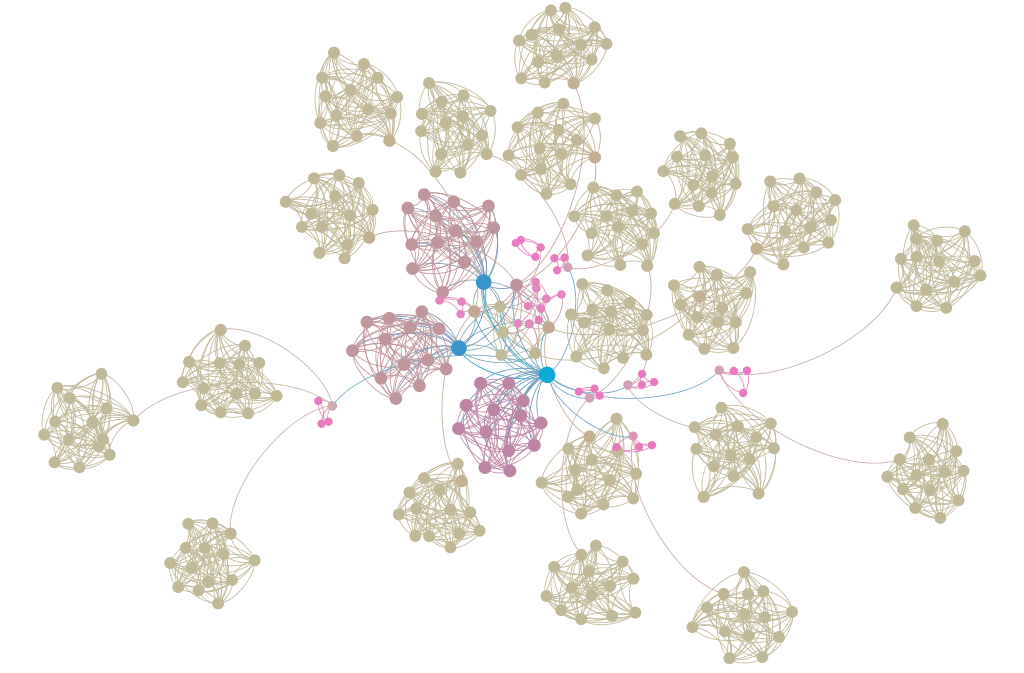
\includegraphics[width=0.7\textwidth]{fig/inf-net.png}
\caption{Information Network for ICM}
\end{figure}

\end{frame}

%------------------------------------------------
\subsection{Task Requirements}
\begin{frame}
\frametitle{Task Requirements}
\begin{columns}[c]
\column{.30\textwidth}
\begin{block}{Modeling}
\begin{enumerate}
\item Churn
\item Recruitment
\item Promotion
\end{enumerate}
\end{block}
\column{.30\textwidth}
\begin{block}{Evaluations}
\begin{enumerate}
\item Costs
\item Productivity
\item HR Health
\end{enumerate}
\end{block}
\column{.30\textwidth}
\begin{block}{Extensions}
\begin{enumerate}
\item Team science
\item Multilayer network
\end{enumerate}
\end{block}
\end{columns}
\end{frame}


%------------------------------------------------
\section{Modeling}
%------------------------------------------------
\subsection{Difficulties in Modeling the Churn Process}
\begin{frame}
\frametitle{Difficulties in Modeling the Churn Process}
The churn process in ICM is hard to model because:
\begin{enumerate}
\item Individually, the churn of the employee is affected by employees around them. 员工互相影响。
\item For ICM as a whole, the churn rate should be maintained in a small interval. (eg. around $18\%$) 整体离职率需要保持恒定。
\item Employees on different positions might have different churn rates. 不同职位的员工有不同的离职率。

\end{enumerate}

Too many assumptions on the employees introduces latent factors, which require some serious parameter tuning to obtain a good model. 过多的假设使得模型的隐含变量太多,导致模拟复杂,难以调参。


\end{frame}

%------------------------------------------------
\begin{frame}
\frametitle{A Negative Example}
One example of a model that introduces too much assumptions for the employees:
\begin{enumerate}
\item Each person has a tolerance threshold, which measures the amount of (dis)satisfaction needed for he/she to leave the company. 不满意度上限
\item Each month, the employee increases the dissatisfaction value based on churn of other employees, his/her position, and working experience. 每个月不满意度增加
\item If the dissatisfaction value exceeds the threshold, the employee will leave the company next month. 超过上限则离职
\end{enumerate}
Result: the employees will leave at {\bf an exponential rate}! 员工离职速度越来越快!
\end{frame}
\subsection{Employee Churn - A Probabilistic Perspective}

\begin{frame}
\frametitle{Employee Churn - A Probabilistic Perspective}
Conclusion: Fewer assumptions are better for simulations!
\begin{block}{The Beta-Bernoulli Distribution}
Suppose a random variable $u\in \{0,1\}$ is drawn from a Bernoulli distribution, where $p$ is unknown:
\begin{equation}
u \sim \mathrm{Bernoulli}(u;p)=p^u(1-p)^{1-u}
\end{equation}
Assume an observer wants to estimate parameter $p$ by drawing multiple $u$'s. The individual has a prior estimation on $p$, which is described as a Beta distribution:
\begin{equation}
f(p)\sim \mathrm{Beta}(p;\alpha, \beta) = \frac{p^{\alpha-1}(1-p)^{\beta-1}}{\mathrm{B}(\alpha, \beta)}
\end{equation}
\end{block}
\end{frame}

\begin{frame}
\frametitle{Employee Churn - A Probablistic Prespective}
\begin{block}{Estimating $\alpha$ and $\beta$}
When seeing an outcome of $u=1$, the observer updates the estimation using Bayes' law: 贝叶斯公式
\begin{equation}
f(p)\sim (p^{\alpha - 1}(1-p)^{\beta-1})\cdot p
\end{equation}
which can be viewed as increasing $\alpha$ by $1$. When the observations reaches infinity, $\alpha/\beta=p$, whereas the Beta distribution reduces to $\delta(u-p)$. Also, the increase of observations reduces the variance of the Beta distribution. Integrating out $p$, the observer can estimate that the mean of $u$ equals $\alpha/(\alpha+\beta)$.

\end{block}
\end{frame}
%------------------------------------------------

\begin{frame}
\frametitle{An Analogy}
\begin{table}
\centering
\begin{tabular}{|c|c|}
\hline
Reality of an employee             &  Model \\\hline
\{Leave, Stay\}                    &  $u\in \{0, 1\}$\\
The true inclination to stay       &  $p$ \\
The estimated inclination to stay  & $\alpha/(\alpha+\beta)$ \\
Seeing others leave                & $\beta \uparrow$ \\
Seeing other stay                  & $\alpha \uparrow$ \\
Experience in company              & $\alpha + \beta$ \\
\hline
\end{tabular}
\caption{Describing the reality using Beta-Bernoulli distribution 模型和现实的比较}
\end{table}
\end{frame}
%------------------------------------------------

\begin{frame}{Three Issues}
\textbf{Determining the Prior 确定初始条件(先验)}
\begin{itemize}
\item Given a churn rate $p$, we can easily model the effect of a churn rate of $p$ per year by setting $\beta / (\alpha + \beta) = p / 12$.
\item It is safe to assume that people on high level positions have a larger $(\alpha+\beta)$ compared to others, and their decisions are less volatile.
\end{itemize}
 
\textbf{Updating $\alpha_i^{(t)}$ and $\beta_i^{(t)}$ 确定参数变化} 
\begin{itemize}
\item We normalize the update values, so that every month, an individual's $(\alpha+\beta)$ increases by 1.
\end{itemize}

\textbf{Information Reduction 信息随传播距离减弱} 
\begin{itemize}
\item We reduce the update by $d^2$ if the information takes at least $d$ steps to transmit.
\end{itemize}

\end{frame}

%------------------------------------------------

\begin{frame}{Algorithm}
To summarize, we introduce an algorithm for this process. For every individual $i$:
\begin{itemize}
\item Sample the churn result for month $t$ using hyperparameters $\alpha_{i,t}$ and $\beta_{i,t}$, and determine whether to stay or to leave; 随机采样得到离职结果
\item If $i$ decides to stay, initialize two variables $\hat{\alpha}$ and $\hat{\beta}$ for update; 
\item For every individual $j$ in $\Gamma^{(t)} \backslash \Theta^{(t)}$(individuals who stays), update $\hat{\alpha} = \hat{\alpha} + \frac{1}{(d_{ij}^{(t)})^2}$;
\item For every individual $j$ in $\Omega^{(t)}$, update $ \hat{\beta} = \hat{\beta} + \frac{1}{(d_{ij}^{(t)})^2}$;
\item Update $ \alpha_{i}^{(t+1)}=\alpha_{i}^{(t)}+\frac{\hat{\alpha}}{\hat{\alpha}+\hat{\beta}}$, and $ \beta_{i}^{(t+1)}=\beta_{i}^{(t)}+\frac{\hat{\beta}}{\hat{\alpha}+\hat{\beta}}$ 根据结果调整参数
\end{itemize}
\end{frame}

\subsection{Modeling HR Manager's Reactions}
\begin{frame}{Promotion Models 晋升模型}
\textbf{Experience Oriented 工作经历优先} \ \ For a vacancy on level $l$, select the employee on level $l+1$ with longest working experiences; the employee should also satisfy the promotion requirements. \vspace{0.5em}

\textbf{Dissatisfaction Oriented 不满意程度优先} \ \  For a vacancy on level $l$, select the employee with the largest $\beta / \alpha$(or the highest churn probability) among all the employees on level $l+1$ who satisfy the promotion requirements. \vspace{0.5em}

\textbf{Centrality Oriented 中心位置优先} \ \ For a vacancy on level $l$, select the employee with the largest closeness centrality (tends to be greater when the employee is in the middle of the network) from the qualified employees on level $l+1$. \vspace{0.5em}

If nobody is available, start recruiting.

\end{frame}

\begin{frame}{Recruitment Models 招聘模型}
Recruitment is implemented using a greedy algorithm: 贪心算法
\begin{itemize}
\item The HR manager has a maximum possible effort to recruit. 同时招聘职位上限
\item When the number of vacant positions is higher than the maximum effort, and only try to recruit the positions with the highest levels. 优先招聘高级员工
\item He can only renew his recruitment post over a length of period, e.g. quarterly or semi-annually. 定期更新招聘职位
\end{itemize}
\end{frame}

\begin{frame}{Capabilities of the Model}
\begin{itemize}
\item The risk of churn can be identified in early stage by observing each staff member's $\beta/\alpha$. The higher $\beta/\alpha$ is, the more likely the staff member chooses to leave. 检测员工离职意愿
\item The resignation of a staff member will increase the $\beta$ parameter of other employees, thus increasing their chance of resigning. 员工的离职会增加其他员工离职的可能
\item We cover the fact that churn rates for middle managers are higher than other levels of positions by allowing different priors $\alpha$ and $\beta$ for different levels. 通过不同先验控制不同的离职率
\item The HR manager can choose recruitment effort, recruitment time period, and promotion threshold to control the recruitment flow. 多种方法控制招聘
\end{itemize}
\end{frame}

\section{Simulations}
\begin{frame}{Task 1}

\begin{figure}
\centering
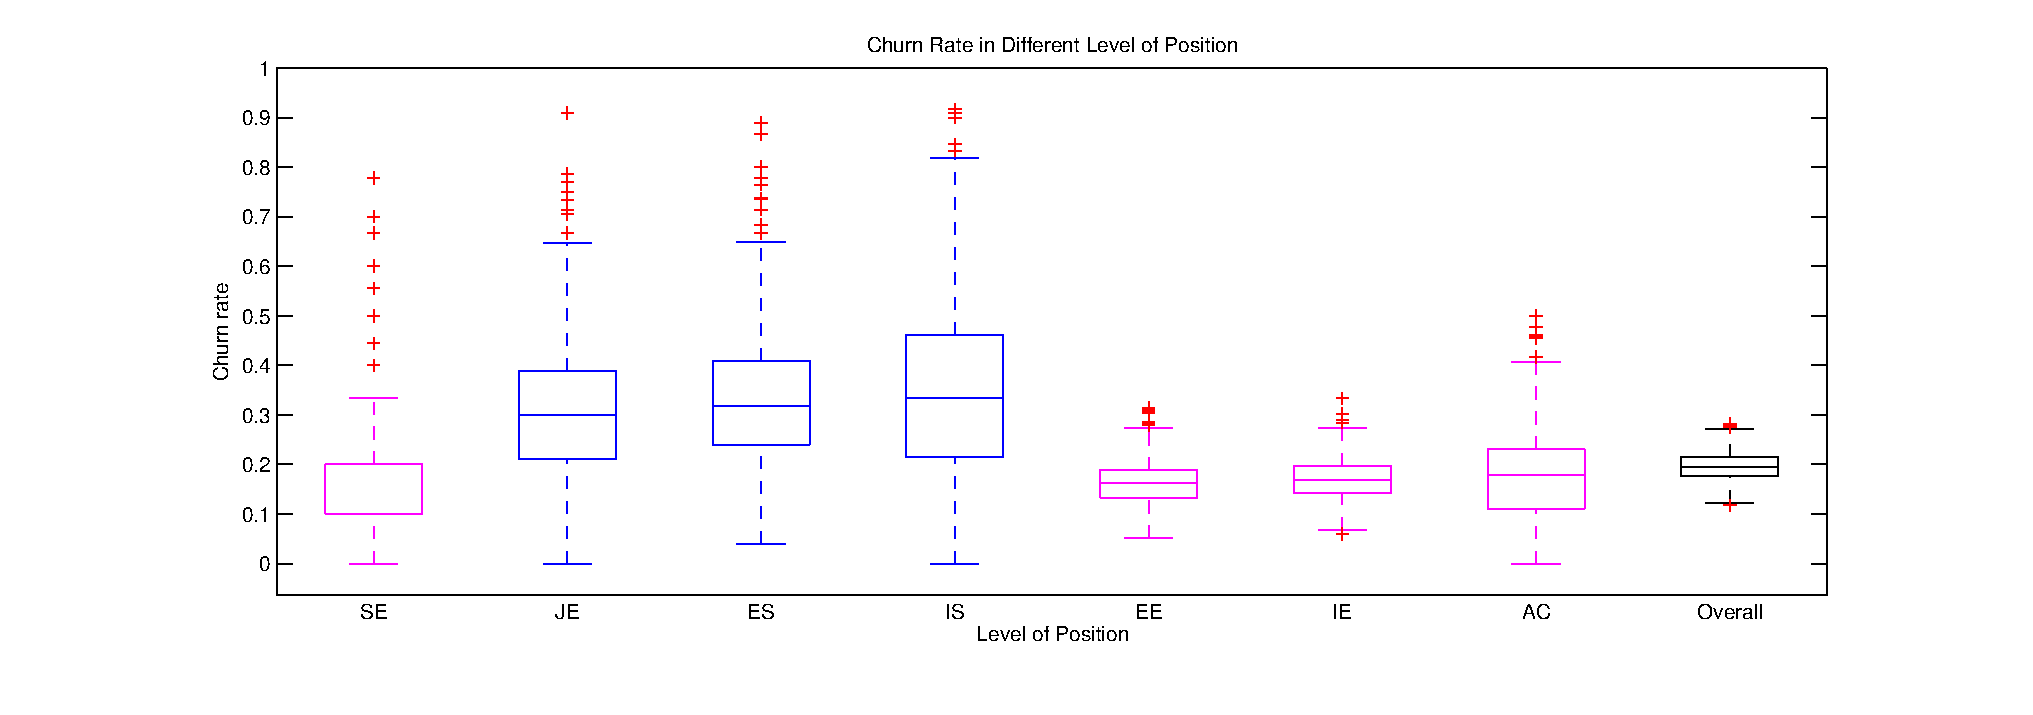
\includegraphics[width=\textwidth]{fig/task-1-1.eps}
\caption{Churn Rate In Different Level of Position}
\end{figure}

\end{frame}

\begin{frame}{Task 1}
\begin{figure}
\centering
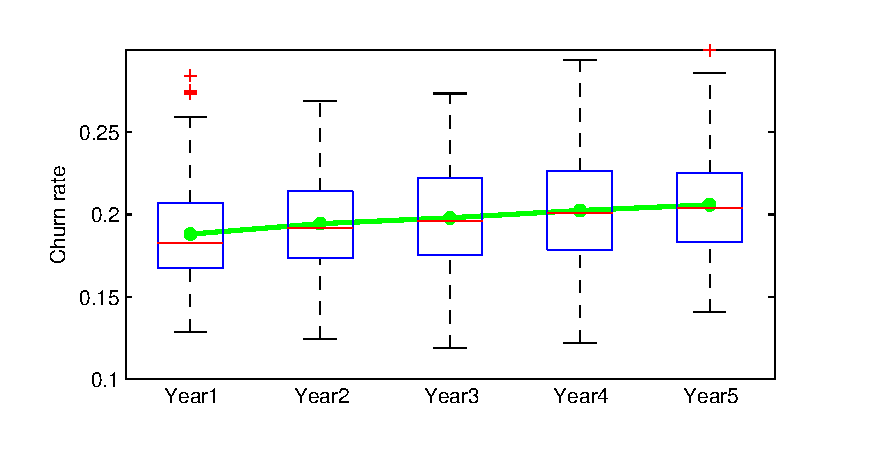
\includegraphics[width=0.8\textwidth]{fig/task-1-2.eps}
\caption{Churn Rate Change over 5 Years}
\end{figure}
\end{frame}

\begin{frame}{Task 2}
We can assume that an employee's productivity is determined by \textbf{position level}, \textbf{training experience}, and \textbf{dissatisfaction}, and that the organizational productivity is a weighted sum of individual productivity. \\\vspace{0.5em}

\textbf{Direct Effect 离职对效率的直接因素}

The productivity of resigned individuals. 离职人员的效率 \vspace{0.5em}

\textbf{Indirect Effect 离职对效率的间接因素}

The loss of productivity caused by the increase of dissatisfaction of the remaining staff in the company after the resignation. 离职人员对其他人员的效率影响


\end{frame}

\begin{frame}{Task 2}
\begin{figure}
\centering
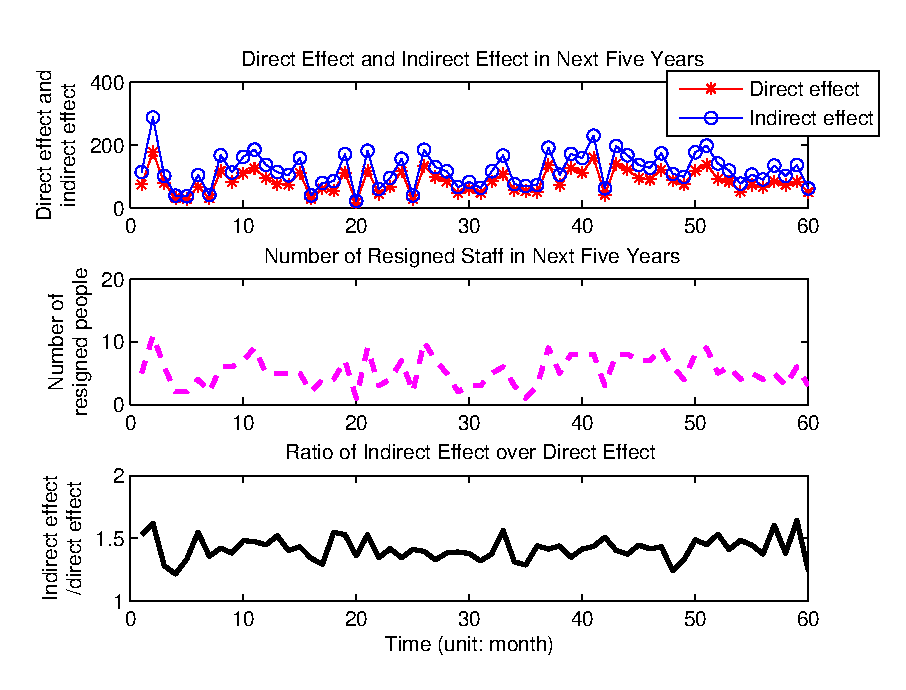
\includegraphics[width=0.70\textwidth]{fig/task-2.eps}
\caption{Direct Effect vs Indirect Effect}
\end{figure}
\end{frame}

\begin{frame}{Task 3}
Budget consists of three components: staff salaries, recruitment cost and training cost.
\begin{columns}
\column{.50\textwidth}
\begin{figure}
\centering
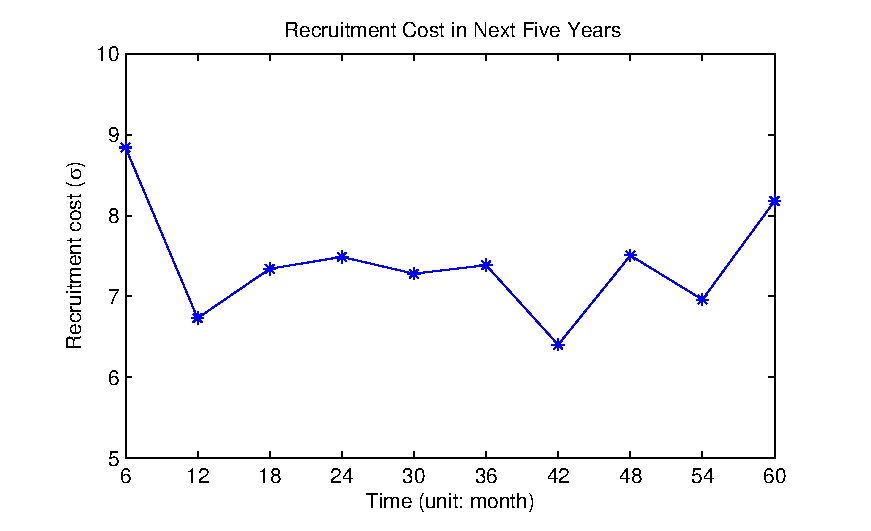
\includegraphics[width=1.0\textwidth]{fig/task-3-1.eps}
\caption{Recruitment Cost}
\end{figure}
\column{.50\textwidth}
\begin{figure}
\centering
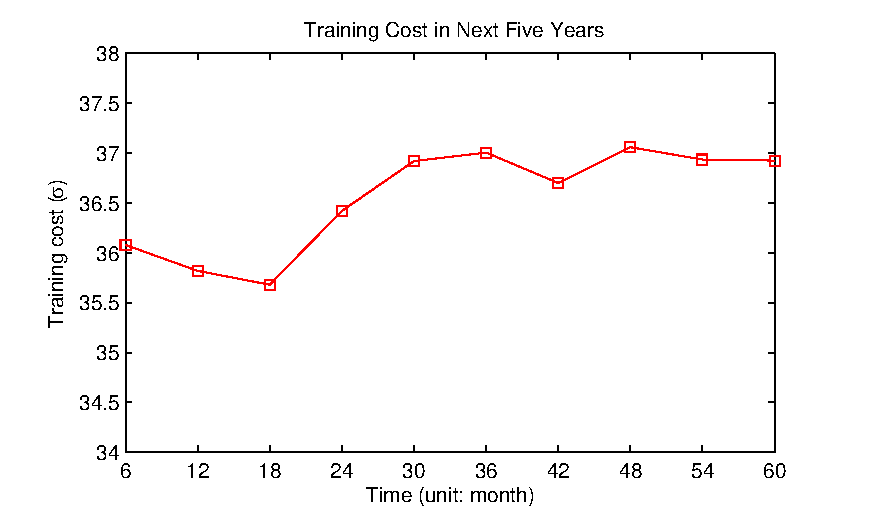
\includegraphics[width=1.0\textwidth]{fig/task-3-2.eps}
\caption{Training Cost}
\end{figure}
\end{columns}

\end{frame}

\begin{frame}{Task 4}
$\beta$-to-$\alpha$ ratio: 
\begin{itemize}
\item Churn rate of 25\% per year, $\beta/\alpha = 0.25/12 = 0.02083$;
\item Churn rate of 35\% per year, $\beta/\alpha = 0.35/12 = 0.02916$.
\end{itemize}


\begin{figure}
\centering
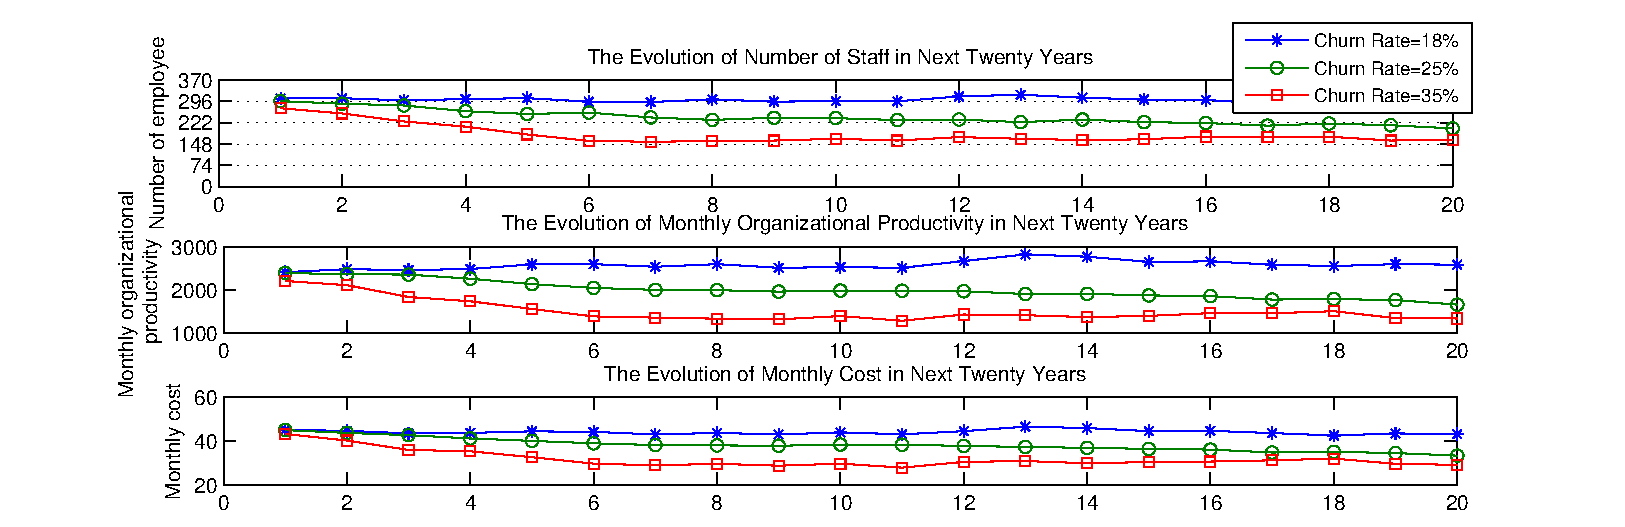
\includegraphics[width=\textwidth]{fig/task-4-1.eps}
\caption{Evolution over the next 20 years}
\end{figure}
\end{frame}

\begin{frame}{Task 4}
\begin{figure}
\centering
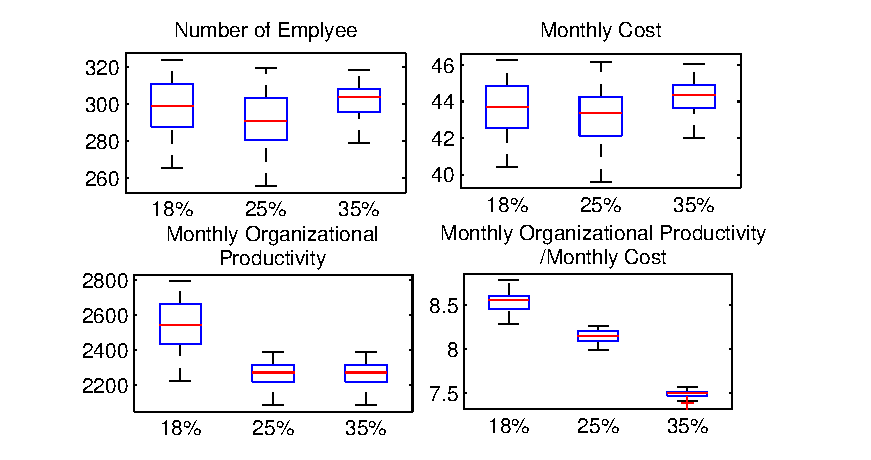
\includegraphics[width=\textwidth]{fig/task-4-2.eps}
\caption{Comparison under different churn rate}
\end{figure}
\end{frame}


\begin{frame}{Task 5}

\begin{columns}
\column{.50\textwidth}
\begin{figure}
\centering
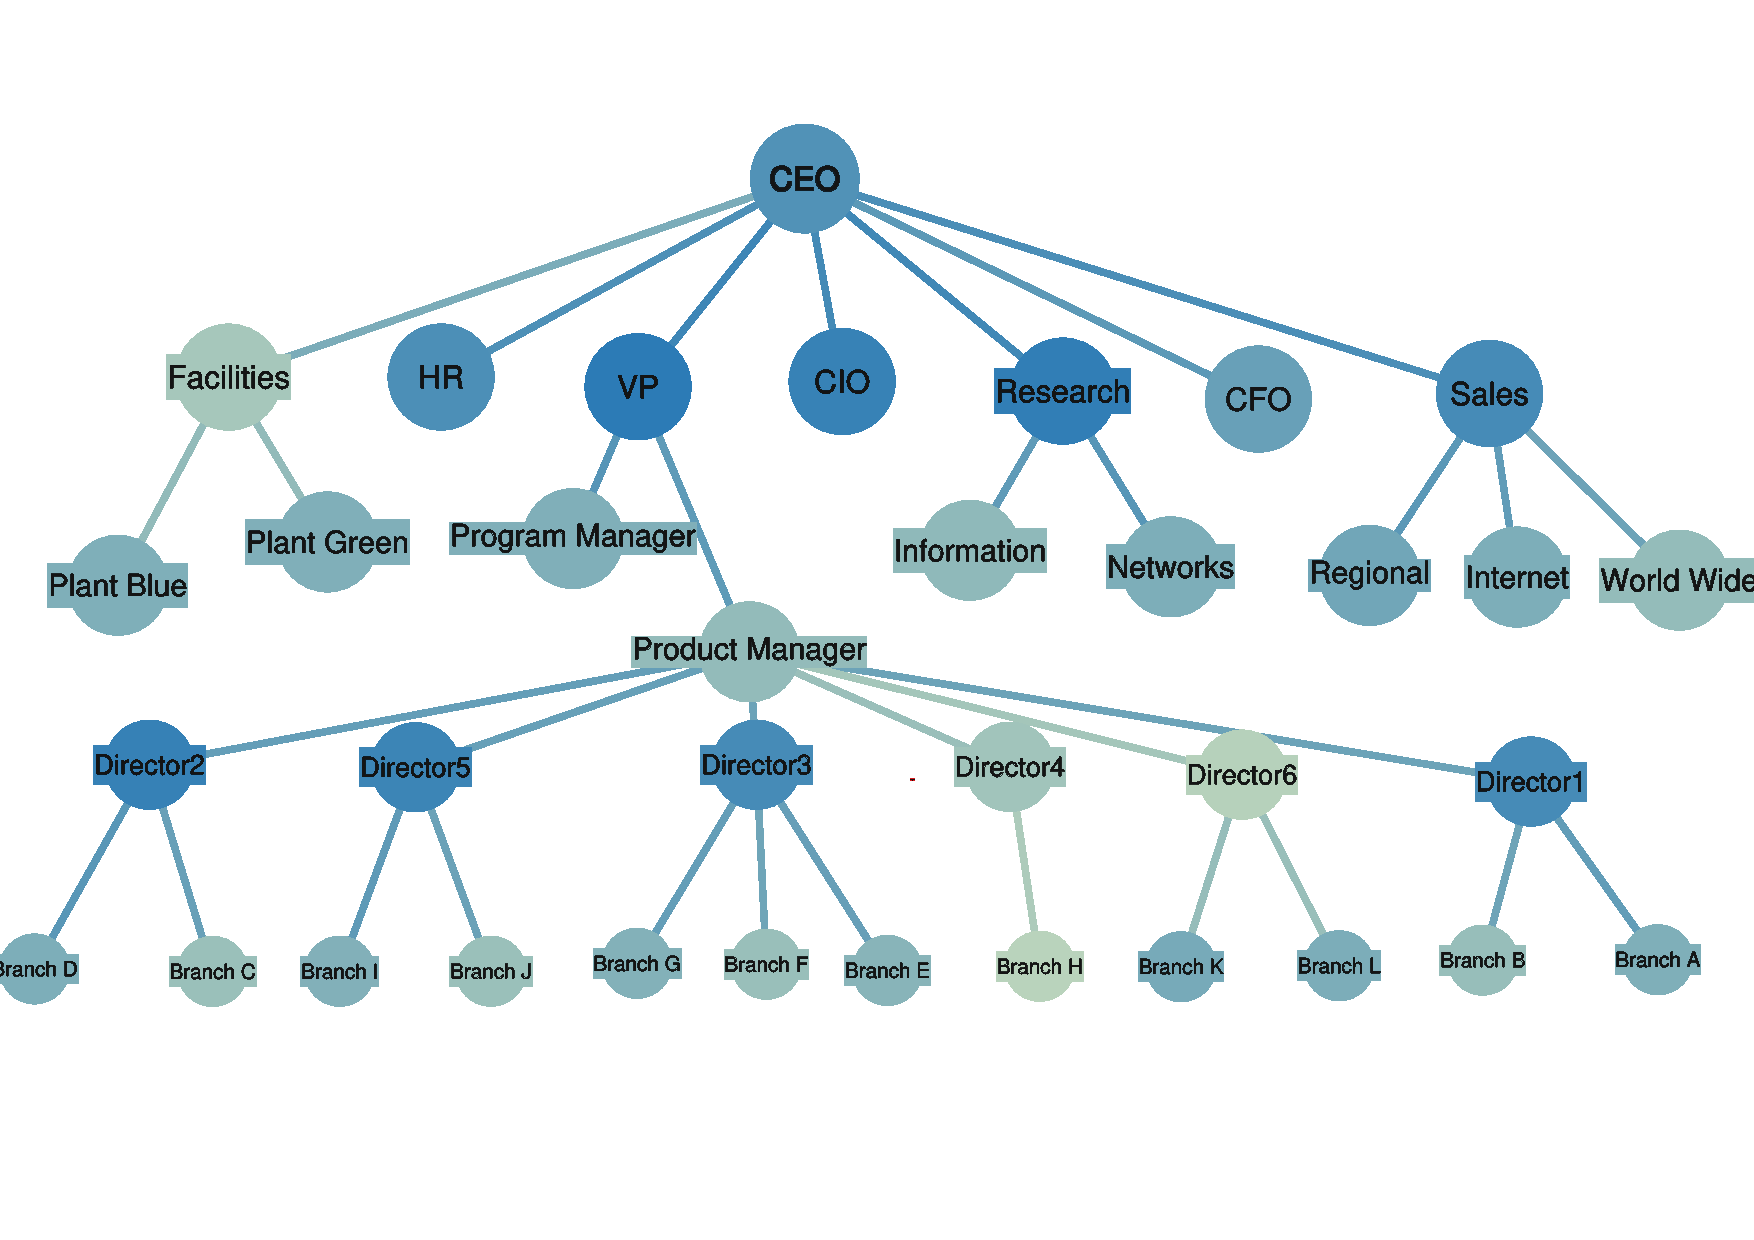
\includegraphics[width=\textwidth]{fig/task-5-1.pdf}
\caption{0 months}
\end{figure}



\column{.50\textwidth}

\begin{figure}
\centering
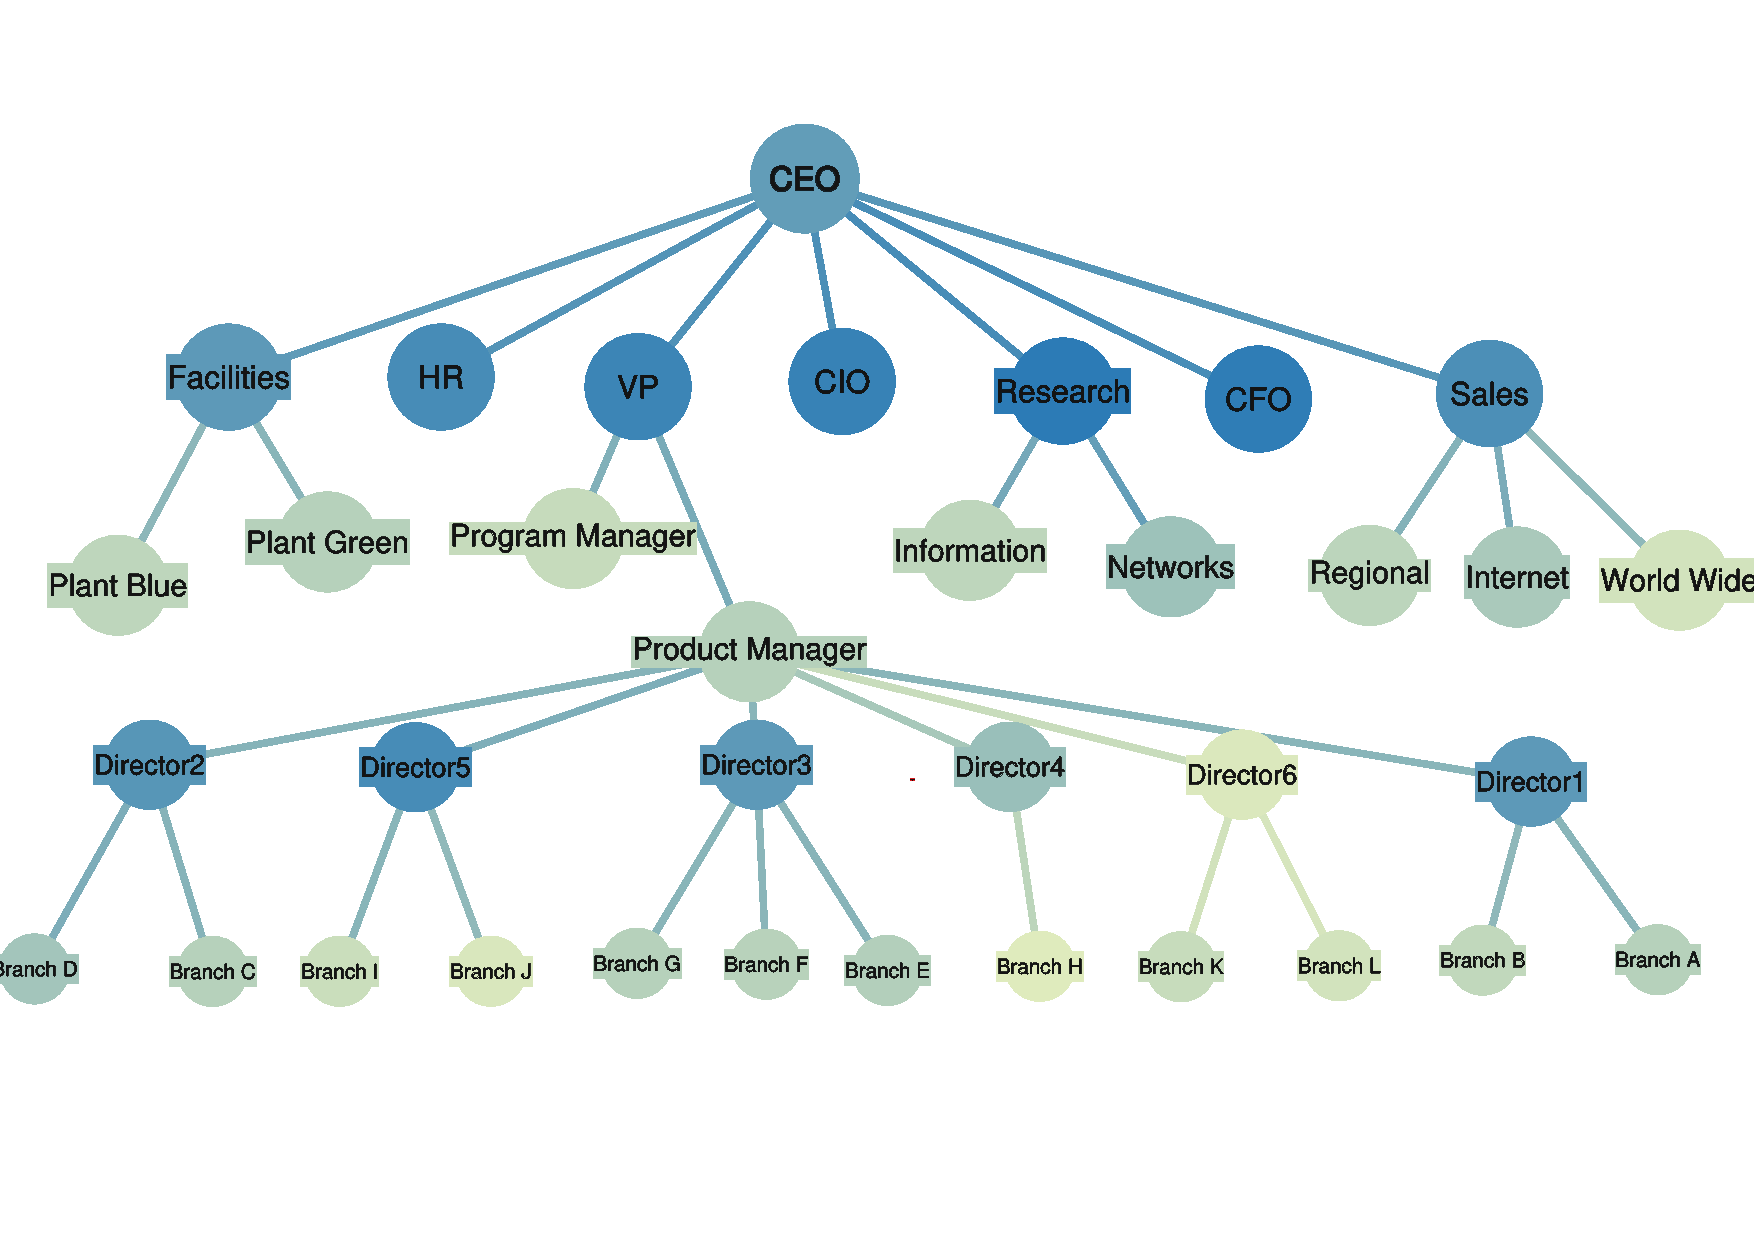
\includegraphics[width=\textwidth]{fig/task-5-2.pdf}
\caption{12 months}
\end{figure}



\end{columns}

\end{frame}

\begin{frame}{Task 5}
\begin{columns}
\column{.50\textwidth}
\begin{figure}
\centering
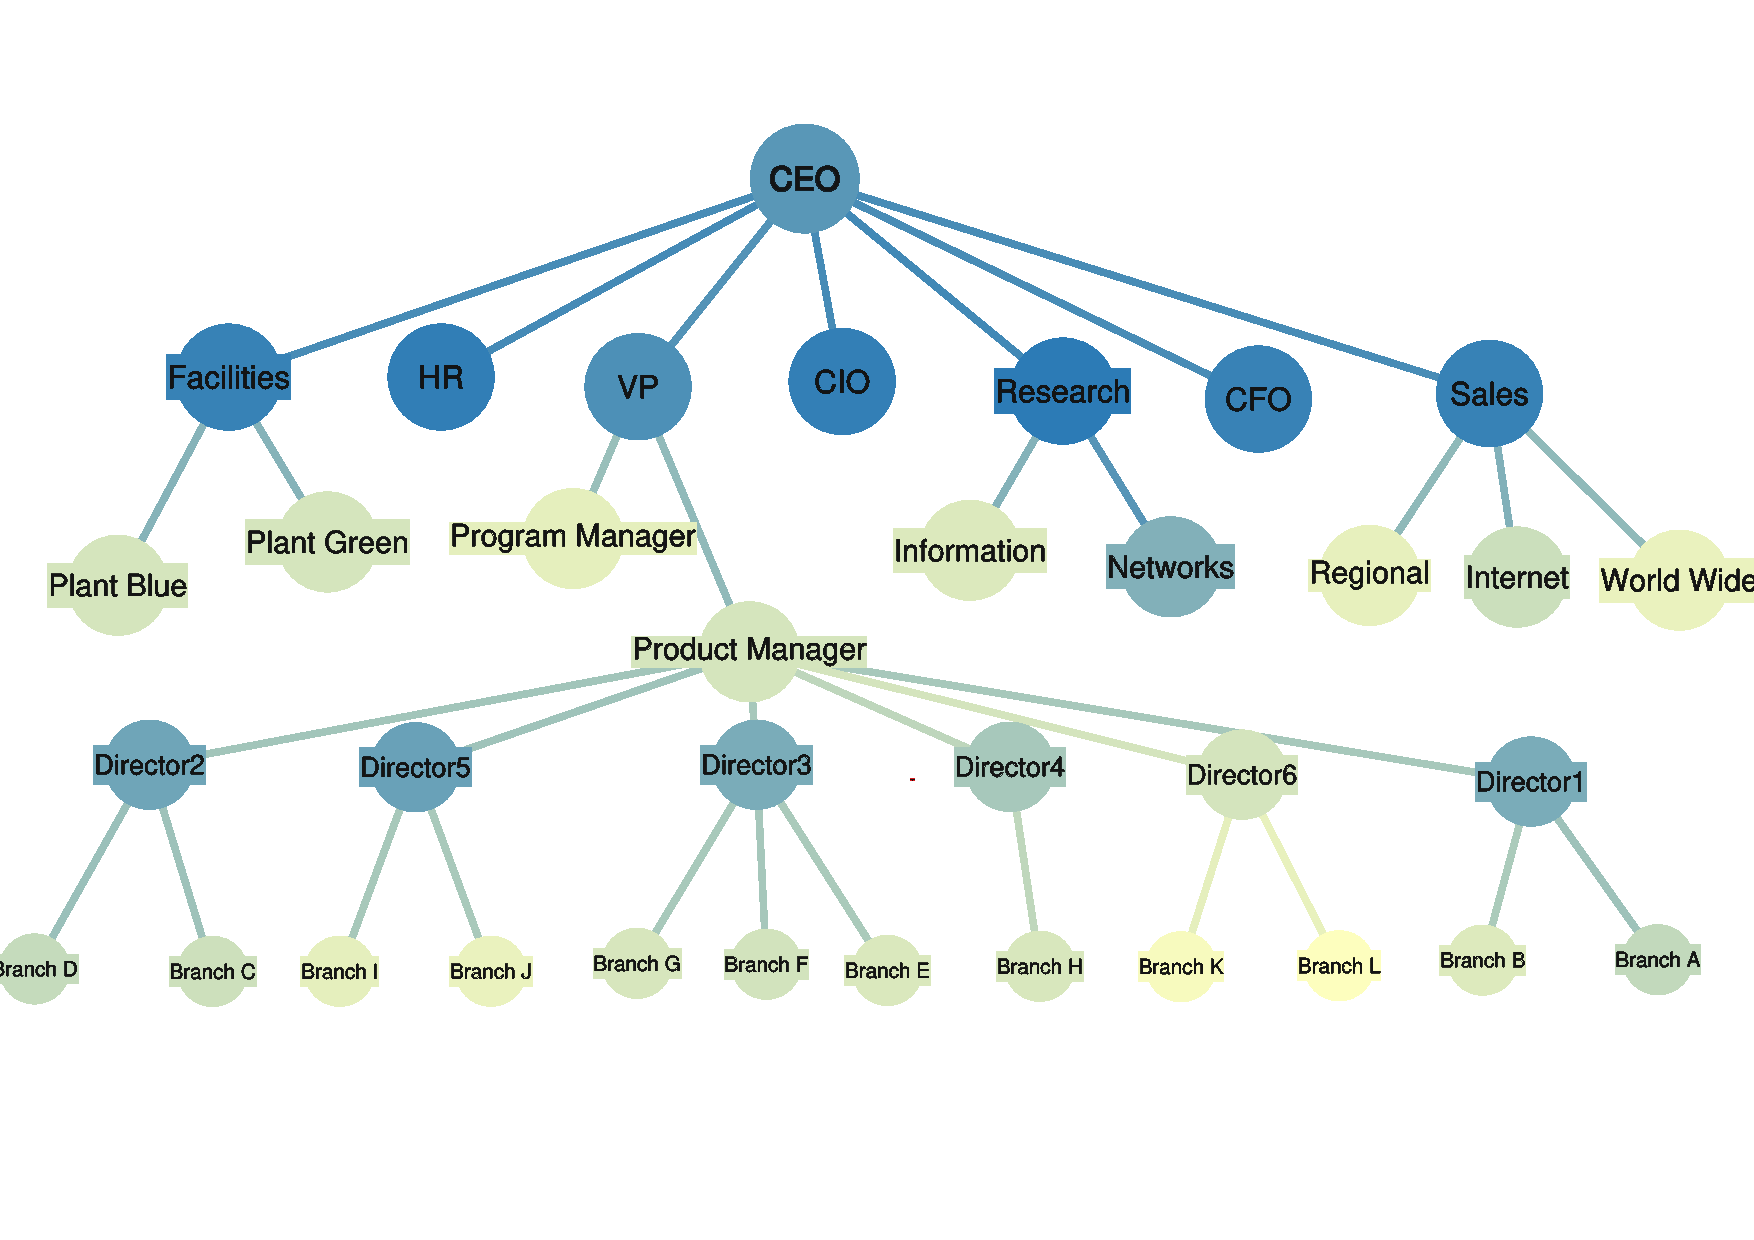
\includegraphics[width=\textwidth]{fig/task-5-3.pdf}
\caption{18 months}
\end{figure}
\column{.5\textwidth}
\begin{figure}
\centering
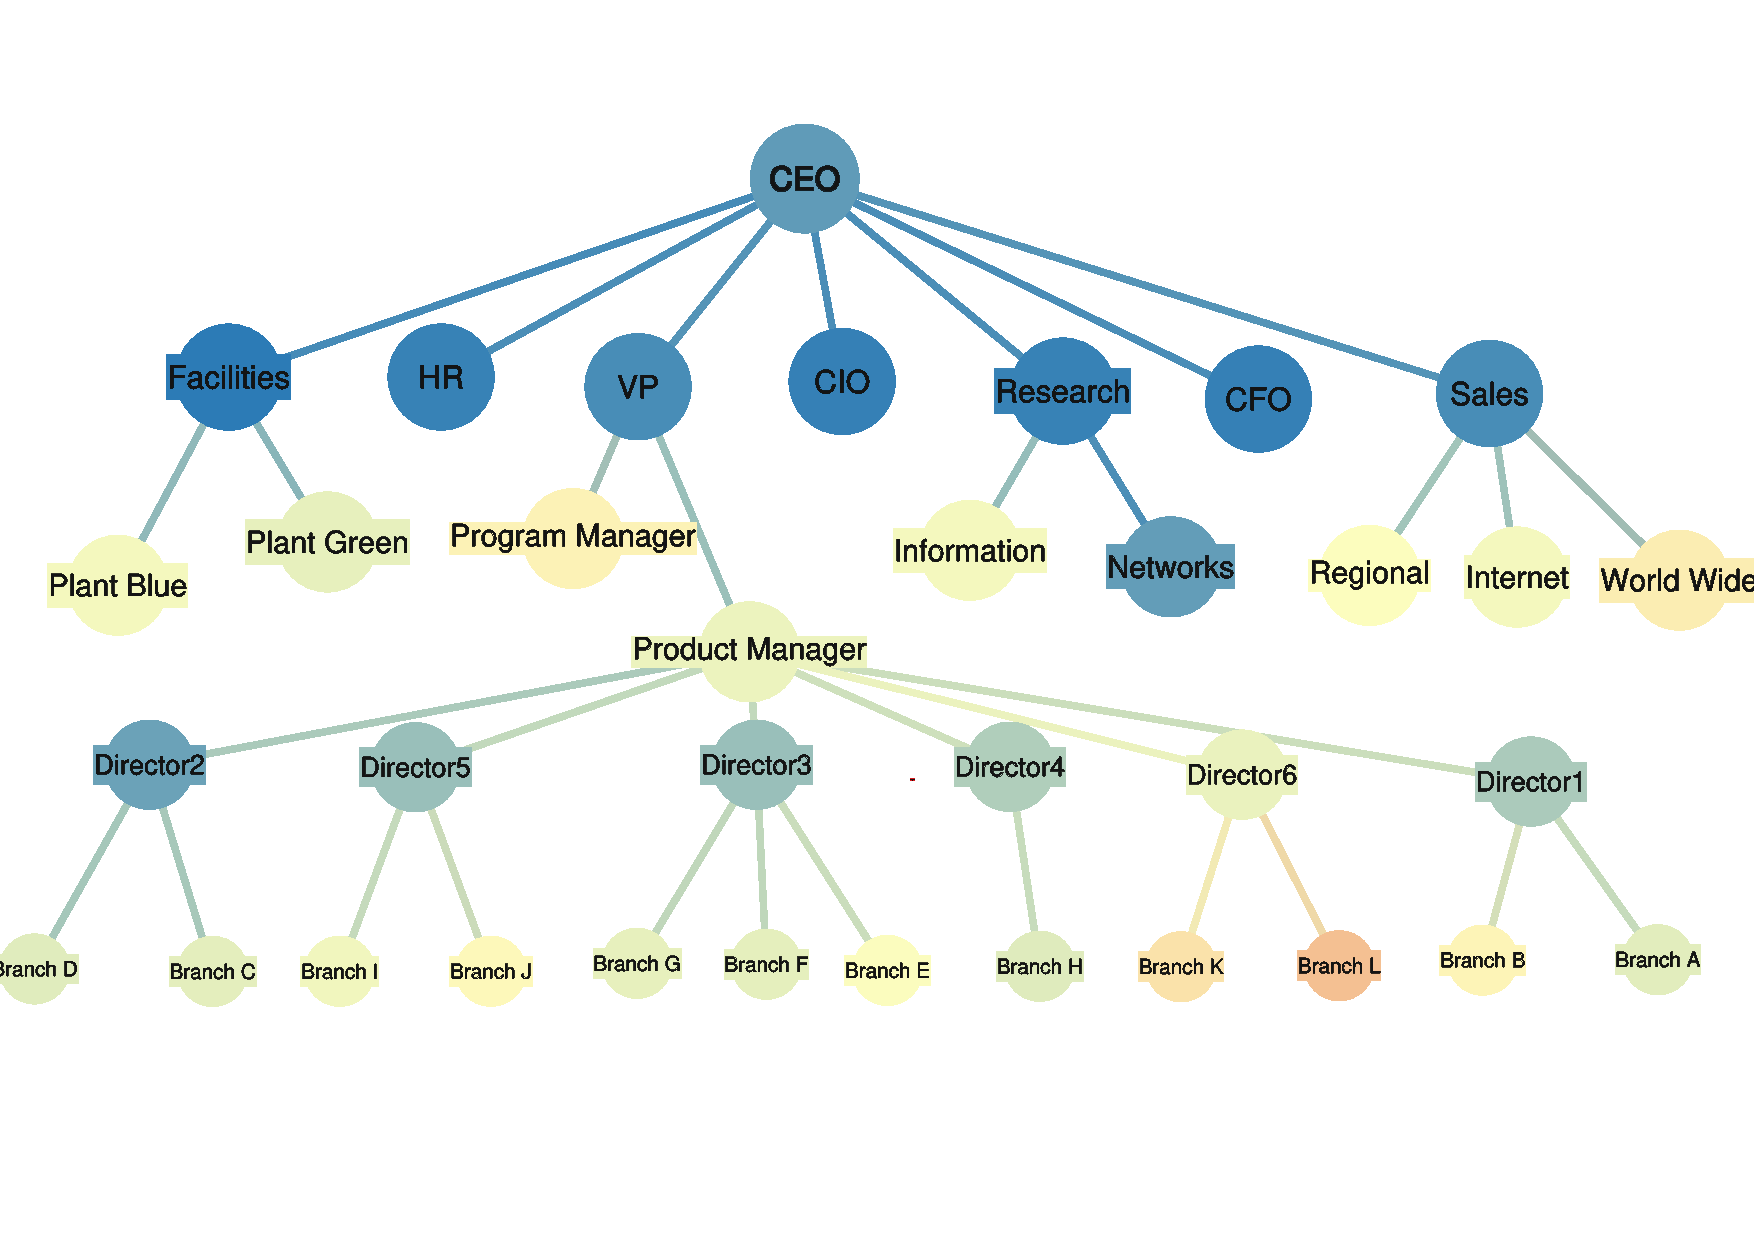
\includegraphics[width=\textwidth]{fig/task-5-4.pdf}
\caption{24 months}
\end{figure}
\end{columns}
\end{frame}

\section{Extensions}
\subsection{Team Science }
\begin{frame}{Incorporating Team Science 团队科学}
\textbf{Shared cognition 共同认知}\ \  Shared cognition can form within different kinds of teams. In our context, a reasonable choice is an office. Staff working within an office share the same goal and shared cognition can positively contribute to its performance.\\\vspace{0.5em}
\textbf{Team Training 团队训练} \ \ Currently, HR manager does not offer any training to the "team" or "office" as a whole. Like offering individual's training, we can take into account the team training. Being trained as a team can improve team members' understanding of each other's roles, promote teamwork and enhance team performance.
\end{frame}

\subsection{Multilayer Networks}
\begin{frame}{Incorporating Multilayer Networks 多层网络}
Now let us assume that we have incorporated teammate, friendship and trust relationship layers to our information network. 队友,友情,信任关系都可以作为多层网络的元素。

\begin{itemize}
\item Churn information can now also transmit along other layers of networks; 通过多种网络传输
\item We reduce our time slice from one month to a week, which allows more frequent information transmission between friends and teammates; 更快的信息传播周期
\item We increase the impact of turnover decisions made by trusted individuals; 增加被信任的人离职的影响
\item We take friendship into account when calculating shared cognition, where friends in the same office tend to have increased shared cognition, and hence productivity. 友情可以增加效率

\end{itemize}

\end{frame}

\subsection{Strengths and Weaknesses}

\begin{frame}{Strengths}
\begin{itemize}
\item \textbf{Simplicity 假设合理}: We make minimum assumptions on individual characteristics: only $\alpha$ and $\beta$ are required for inference. 
\item \textbf{Parameters 参数简单}: The parameters reduce the need of tuning to a minimum.
\item \textbf{Coverage 应用广泛}: Our model and measures are capable of simulating various scenarios.
\item \textbf{Flexibility 灵活扩展}: Our model can be easily incorporated with other assumptions.
\item \textbf{Appealing simulation results 结果优美}: Simulation results of our model are very appealing.  
\item \textbf{Heuristics for HR 管理经验}: HR can gain considerable heuristics from our paper.
\end{itemize}
\end{frame}

\begin{frame}{Weaknessses}
\begin{itemize}
\item \textbf{Simulation volatility 仿真波动剧烈}: Although our model has nice statistical properties, results generated by different simulations suffer high volatility. One possible remedy is to increase the sampling time, which reduces outcome variance at the cost of computational resources.

\item \textbf{Unrealistic assumptions 部分假设}: Some of our measures are based on unrealistic foundations, e.g. productivity increases linearly with training costs, employees have no inclination towards different positions, etc.

\item \textbf{Incomplete assumptions 部分假设缺失}: There are also some other perspectives where we fail to consider, such as the positive effects of team cognition on productivity. 
\end{itemize}
\end{frame}

\begin{frame}{More Information}
For the paper, please visit \url{https://github.com/jiamings/icm2015}. \\\vspace{0.5em}

My contact information:
\begin{itemize}
\item Name: Jiaming Song 宋佳铭
\item Email: jiaming.tsong@gmail.com
\item Mobile: 18001585905
\item WeChat: dipndet
\end{itemize}

\end{frame}
\end{CJK*}
\end{document}
